%==============================================================================
% MATH 110 - Section 1B Notes: Definition of Vector Space
% Linear Algebra Done Right, 4th ed. - Sheldon Axler
%==============================================================================

\documentclass[10pt, twocolumn]{article}
\usepackage[margin=0.75in, columnsep=0.3in]{geometry}

%------------------------------------------------------------------------------
% PACKAGES
%------------------------------------------------------------------------------
\usepackage{amsmath, amssymb, amsthm}
\usepackage{enumitem}
\usepackage{fancyhdr}
\usepackage{titlesec}
\usepackage{tcolorbox}
\tcbuselibrary{breakable}
\usepackage{booktabs}
\usepackage{tikz}
\usetikzlibrary{matrix, arrows.meta, positioning, calc, cd, shapes.geometric}
\usepackage{graphicx}

% TikZ style definitions for consistent diagrams (matching notes-1a)
\tikzset{
    vector/.style={->, >=Stealth, thick},
    axis/.style={->, thin},
    point/.style={fill, circle, inner sep=1.5pt}
}

%------------------------------------------------------------------------------
% SPACING
%------------------------------------------------------------------------------
\linespread{1.08}
\setlength{\parskip}{0.4ex plus 0.2ex minus 0.1ex}

%------------------------------------------------------------------------------
% BOX STYLES
%------------------------------------------------------------------------------
\tcbset{
    boxrule=0.8pt,
    colback=white,
    colframe=black,
    arc=0pt,
    boxsep=3pt,
    left=4pt, right=4pt, top=4pt, bottom=4pt,
    breakable
}

\newtcolorbox{result}{
    boxrule=0pt,
    colback=black!5,
    colframe=white,
    arc=0pt,
    boxsep=2pt,
    left=4pt, right=4pt, top=4pt, bottom=4pt,
    breakable
}

%------------------------------------------------------------------------------
% SECTION FORMATTING
%------------------------------------------------------------------------------
\titleformat{\section}{\large\bfseries}{\thesection.}{0.5em}{}
\titleformat{\subsection}{\normalsize\bfseries}{\thesubsection}{0.5em}{}
\titlespacing*{\section}{0pt}{1.5ex}{1ex}
\titlespacing*{\subsection}{0pt}{1ex}{0.5ex}

%------------------------------------------------------------------------------
% LIST FORMATTING
%------------------------------------------------------------------------------
\setlist{itemsep=1pt, topsep=3pt, parsep=1pt, leftmargin=1.5em}

%------------------------------------------------------------------------------
% HEADER/FOOTER
%------------------------------------------------------------------------------
\pagestyle{fancy}
\fancyhf{}
\fancyhead[L]{\small MATH 110}
\fancyhead[R]{\small Section 1B}
\fancyfoot[C]{\small\thepage}
\renewcommand{\headrulewidth}{0.4pt}

%------------------------------------------------------------------------------
% THEOREM ENVIRONMENTS
%------------------------------------------------------------------------------
\theoremstyle{definition}
\newtheorem{property}{Property}
\newtheorem{definition}{Definition}
\newtheorem{example}{Example}

\theoremstyle{plain}
\newtheorem{theorem}{Theorem}
\newtheorem{lemma}{Lemma}
\newtheorem{proposition}{Proposition}
\newtheorem{corollary}{Corollary}

%------------------------------------------------------------------------------
% CUSTOM COMMANDS
%------------------------------------------------------------------------------
% Number fields
\newcommand{\R}{\mathbb{R}}
\newcommand{\C}{\mathbb{C}}
\newcommand{\F}{\mathbb{F}}
\newcommand{\Z}{\mathbb{Z}}
\newcommand{\Q}{\mathbb{Q}}

% Matrix/space operations
\DeclareMathOperator{\rank}{rank}
\DeclareMathOperator{\nullity}{nullity}
\DeclareMathOperator{\tr}{tr}
\DeclareMathOperator{\spn}{span}
\DeclareMathOperator{\col}{col}
\DeclareMathOperator{\row}{row}
\DeclareMathOperator{\nul}{null}
\DeclareMathOperator{\range}{range}
\DeclareMathOperator{\im}{im}

% Inner products and norms
\newcommand{\inner}[2]{\langle #1, #2 \rangle}
\newcommand{\norm}[1]{\| #1 \|}
\newcommand{\proj}{\operatorname{proj}}

% Vectors and matrices
\newcommand{\vect}[1]{\mathbf{#1}}
\newcommand{\mat}[1]{\mathbf{#1}}

%==============================================================================
\begin{document}
%==============================================================================

\noindent
\begin{minipage}{\linewidth}
    \centering
    \textbf{\Large Section 1B: Definition of Vector Space} \\[0.5em]
    \hrule
\end{minipage}
\vspace{1em}

%==============================================================================
\section{Addition and Scalar Multiplication}
%==============================================================================

In Section 1A, we defined addition and scalar multiplication on $\F^n$. Now we abstract these operations to define vector spaces in general.

\begin{tcolorbox}
\textbf{1.19 Definition: Addition, Scalar Multiplication}

\begin{itemize}
    \item An \textbf{addition} on a set $V$ is a function that assigns an element $u + v \in V$ to each pair of elements $u, v \in V$.
    \item A \textbf{scalar multiplication} on a set $V$ is a function that assigns an element $\lambda v \in V$ to each $\lambda \in \F$ and each $v \in V$.
\end{itemize}
\end{tcolorbox}

\textbf{Key point:} Addition takes two elements of $V$ and produces an element of $V$. Scalar multiplication takes a scalar from $\F$ and an element of $V$, producing an element of $V$. These are \textit{functions}: every input has exactly one output.

\textbf{Notation:} We will also use juxtaposition for scalar multiplication: $\lambda v$ means the same as $\lambda \cdot v$.

%==============================================================================
\section{Definition of Vector Space}
%==============================================================================

The following definition is the central definition of linear algebra.

\begin{tcolorbox}
\textbf{1.20 Definition: Vector Space}

A \textbf{vector space} is a set $V$ along with an addition on $V$ and a scalar multiplication on $V$ such that the following properties hold:

\textbf{commutativity:}
\[
    u + v = v + u \quad \text{for all } u, v \in V
\]

\textbf{associativity:}
\[
    (u + v) + w = u + (v + w) \text{ and } (ab)v = a(bv)
\]
for all $u, v, w \in V$ and all $a, b \in \F$

\textbf{additive identity:}
there exists an element $0 \in V$ such that $v + 0 = v$ for all $v \in V$

\textbf{additive inverse:}
for every $v \in V$, there exists $w \in V$ such that $v + w = 0$

\textbf{multiplicative identity:}
\[
    1v = v \quad \text{for all } v \in V
\]

\textbf{distributive properties:}
\[
    a(u + v) = au + av \text{ and } (a + b)v = av + bv
\]
for all $a, b \in \F$ and all $u, v \in V$
\end{tcolorbox}

\begin{tcolorbox}
\textbf{1.21 Definition: Vector, Point}

Elements of a vector space are called \textbf{vectors} or \textbf{points}.
\end{tcolorbox}

\textbf{Terminology:} The elements of $\F$ are called \textbf{scalars}. The word ``scalar'' is used because elements of $\F$ scale vectors via scalar multiplication.

\begin{tcolorbox}
\textbf{1.22 Definition: Real Vector Space, Complex Vector Space}

\begin{itemize}
    \item A vector space over $\R$ is called a \textbf{real vector space}.
    \item A vector space over $\C$ is called a \textbf{complex vector space}.
\end{itemize}
\end{tcolorbox}

\textbf{Note:} The simplest vector space is $\{0\}$, which contains only the additive identity.

\begin{result}
\textbf{Mnemonic for the 8 axioms:} ``CAAIMD$^2$''
\begin{itemize}
    \item \textbf{C}ommutativity of addition
    \item \textbf{A}ssociativity of addition
    \item \textbf{A}ssociativity of scalar multiplication
    \item Additive \textbf{I}dentity
    \item Additive inverse (``\textbf{I}nverse'')
    \item \textbf{M}ultiplicative identity
    \item \textbf{D}istributive (scalar over vector sum)
    \item \textbf{D}istributive (scalar sum over vector)
\end{itemize}
\end{result}

\begin{result}
\textbf{Why These Axioms? (Geometric Intuition)}

These axioms aren't arbitrary; each captures an essential geometric property:

\textbf{Commutativity \& Associativity:} The parallelogram rule for adding vectors works regardless of which vector you draw first. Moving ``3 steps east then 2 north'' reaches the same point as ``2 north then 3 east.''

\smallskip
\begin{center}
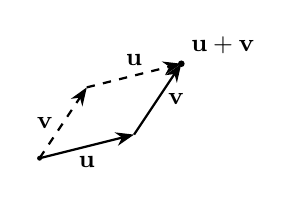
\begin{tikzpicture}[scale=0.6]
    \fill (0,0) circle (1.5pt);
    \draw[vector] (0,0) -- (2,0.5) node[midway, below] {\small$\mathbf{u}$};
    \draw[vector] (2,0.5) -- (3,2) node[midway, right] {\small$\mathbf{v}$};
    \draw[vector, dashed] (0,0) -- (1,1.5) node[midway, left] {\small$\mathbf{v}$};
    \draw[vector, dashed] (1,1.5) -- (3,2) node[midway, above] {\small$\mathbf{u}$};
    \fill (3,2) circle (2pt) node[above right] {\small$\mathbf{u}+\mathbf{v}$};
\end{tikzpicture}
\end{center}

\textbf{Additive Identity \& Inverse:} We need a ``do nothing'' operation ($0$) and a way to ``undo'' addition ($-v$). Geometrically: the origin exists, and every direction has an opposite.

\textbf{Multiplicative Identity:} Scaling by 1 leaves a vector unchanged. This anchors our notion of ``unit scale.''

\textbf{Distributive Laws:} Scaling respects the structure of addition. Stretching $\mathbf{u} + \mathbf{v}$ by factor $\lambda$ is the same as stretching each separately, then adding.
\end{result}

%==============================================================================
\section{Examples of Vector Spaces}
%==============================================================================

The set $\F^n$ with the addition and scalar multiplication defined in Section 1A is a vector space over $\F$. We verified commutativity in Section 1A; the other vector space properties follow similarly by working coordinate-by-coordinate.

\begin{tcolorbox}[colframe=black!50]
\textbf{1.23 Example: $\F^\infty$}

Define $\F^\infty$ as the set of all sequences of elements of $\F$:
\[
    \F^\infty = \{(x_1, x_2, x_3, \ldots) : x_k \in \F \text{ for } k = 1, 2, \ldots\}
\]

Addition and scalar multiplication are defined coordinate-wise:
\begin{align*}
    (x_1, x_2, \ldots) + (y_1, y_2, \ldots) &= (x_1 + y_1, x_2 + y_2, \ldots) \\
    \lambda(x_1, x_2, \ldots) &= (\lambda x_1, \lambda x_2, \ldots)
\end{align*}

With these operations, $\F^\infty$ is a vector space over $\F$.
\end{tcolorbox}

\textbf{Intuition:} $\F^\infty$ is like $\F^n$ but with infinitely many coordinates. The verification is identical; each axiom is checked coordinate-wise.

\begin{result}
\textbf{The Abstraction Ladder: From $\F^n$ to $\F^S$}

We've now seen two vector spaces with similar structure:
\begin{itemize}
    \item $\F^n$: lists indexed by $\{1, 2, \ldots, n\}$
    \item $\F^\infty$: sequences indexed by $\Z^+ = \{1, 2, 3, \ldots\}$
\end{itemize}

What do these have in common? In both cases, we have a set of ``indices'' ($\{1, \ldots, n\}$ or $\Z^+$), and a vector assigns a scalar to each index. This leads to a powerful abstraction: what if we index by \textit{any} set $S$?
\end{result}

\begin{tcolorbox}
\textbf{1.24 Notation: $\F^S$}

If $S$ is a nonempty set, then $\F^S$ denotes the set of all functions from $S$ to $\F$.

For $f, g \in \F^S$, the \textbf{sum} $f + g \in \F^S$ is the function defined by
\[
    (f + g)(x) = f(x) + g(x)
\]
for all $x \in S$.

For $\lambda \in \F$ and $f \in \F^S$, the \textbf{product} $\lambda f \in \F^S$ is the function defined by
\[
    (\lambda f)(x) = \lambda f(x)
\]
for all $x \in S$.
\end{tcolorbox}

\begin{tcolorbox}[colframe=black!50]
\textbf{1.25 Example: $\F^S$ is a Vector Space}

If $S$ is a nonempty set, then $\F^S$ (with the operations of addition and scalar multiplication as defined in 1.24) is a vector space over $\F$.

\textbf{Details:}
\begin{itemize}
    \item The additive identity of $\F^S$ is the function $0: S \to \F$ defined by $0(x) = 0$ for all $x \in S$.
    \item For $f \in \F^S$, the additive inverse of $f$ is the function $-f: S \to \F$ defined by $(-f)(x) = -f(x)$ for all $x \in S$.
\end{itemize}
\end{tcolorbox}

\textbf{Key insight:} The ``vectors'' in $\F^S$ are \textit{functions}. Addition means adding function values pointwise.

\textbf{Why functions are vectors:} This may seem abstract, but it's incredibly powerful. A function $f: S \to \F$ assigns a number to each point in $S$---just like a tuple $(x_1, \ldots, x_n)$ assigns a number to each index. The key realization is that \textit{any} way of assigning numbers to a collection of labels can be viewed as a vector. This viewpoint unifies:
\begin{itemize}
    \item Polynomials (coefficients indexed by degree)
    \item Signals (amplitude indexed by time)
    \item Images (pixel values indexed by position)
\end{itemize}

\smallskip
\begin{center}
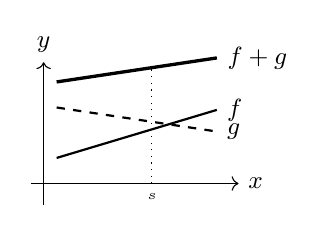
\begin{tikzpicture}[scale=0.55]
    % Axes
    \draw[axis] (-0.3,0) -- (4.5,0) node[right] {\small$x$};
    \draw[axis] (0,-0.5) -- (0,2.8) node[above] {\small$y$};
    % Function f
    \draw[thick, domain=0.3:4, samples=50] plot (\x, {0.3*\x + 0.5}) node[right] {\small$f$};
    % Function g
    \draw[thick, dashed, domain=0.3:4, samples=50] plot (\x, {-0.15*\x + 1.8}) node[right] {\small$g$};
    % Function f+g
    \draw[very thick, domain=0.3:4, samples=50] plot (\x, {0.15*\x + 2.3}) node[right] {\small$f+g$};
    % Vertical line showing pointwise addition
    \draw[dotted] (2.5,0) -- (2.5,2.68);
    \node[below] at (2.5,0) {\tiny$s$};
\end{tikzpicture}

\small\textit{Pointwise addition: $(f+g)(s) = f(s) + g(s)$}
\end{center}
\smallskip

\begin{result}
\textbf{Unifying perspective:} $\F^n$ is a special case of $\F^S$ where $S = \{1, 2, \ldots, n\}$. A list $(x_1, \ldots, x_n)$ is the same as the function $f: \{1, \ldots, n\} \to \F$ defined by $f(k) = x_k$.

Similarly, $\F^\infty$ is $\F^S$ where $S = \Z^+ = \{1, 2, 3, \ldots\}$.
\end{result}

\smallskip
\begin{center}
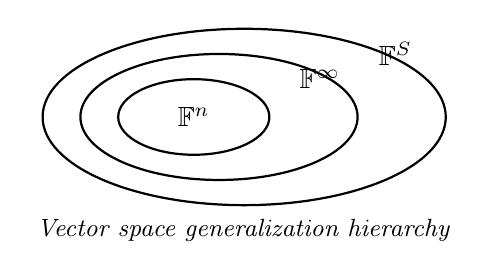
\begin{tikzpicture}[scale=0.8]
    % Nested ellipses
    \draw[thick] (0,0) ellipse (3.2cm and 1.4cm);
    \node at (2.4,1.0) {$\F^S$};
    \draw[thick] (-0.4,0) ellipse (2.2cm and 1.0cm);
    \node at (1.2,0.6) {$\F^\infty$};
    \draw[thick] (-0.8,0) ellipse (1.2cm and 0.6cm);
    \node at (-0.8,0) {$\F^n$};
    % Labels below
    \node at (0,-1.8) {\small\textit{Vector space generalization hierarchy}};
\end{tikzpicture}
\end{center}
\smallskip

%==============================================================================
\section{Uniqueness Results}
%==============================================================================

\textbf{Geometric intuition:} The axioms guarantee that additive identities and inverses \textit{exist}, but why should they be \textit{unique}? Geometrically, if there were two different ``origins'' in our space, we'd have two incompatible reference points---vectors would have ambiguous positions. Similarly, if a vector had multiple additive inverses, the notion of ``opposite direction'' would be ill-defined. Uniqueness ensures our geometric intuition is well-founded.

\begin{result}
\textbf{Proof Technique: Uniqueness Arguments}

To prove an object is unique:
\begin{enumerate}
    \item Assume two objects satisfy the defining property
    \item Show they must be equal using that property
\end{enumerate}
This ``assume two, show equal'' pattern appears throughout mathematics.
\end{result}

The axioms guarantee existence of additive identities and inverses, but we should verify they are unique.

\begin{tcolorbox}
\textbf{1.26 Unique Additive Identity}

A vector space has a unique additive identity.
\end{tcolorbox}

\textbf{Proof:} Suppose $0$ and $0'$ are both additive identities for $V$. Then:
\[
    0' = 0' + 0 = 0 + 0' = 0
\]
The first equality holds because $0$ is an additive identity. The second uses commutativity. The third holds because $0'$ is an additive identity. \hfill $\square$

\begin{tcolorbox}
\textbf{1.27 Unique Additive Inverse}

Every element in a vector space has a unique additive inverse.
\end{tcolorbox}

\textbf{Proof:} Suppose $v \in V$ and both $w$ and $w'$ satisfy $v + w = 0$ and $v + w' = 0$. Then:
\begin{align*}
    w' &= w' + 0 \\
       &= w' + (v + w) \\
       &= (w' + v) + w \\
       &= (v + w') + w \\
       &= 0 + w \\
       &= w
\end{align*}
Thus $w = w'$. \hfill $\square$

\begin{tcolorbox}
\textbf{1.28 Notation: $-v$, $w - v$}

Let $v, w \in V$.
\begin{itemize}
    \item $-v$ denotes the additive inverse of $v$.
    \item $w - v$ is defined by $w - v = w + (-v)$.
\end{itemize}
\end{tcolorbox}

\begin{tcolorbox}
\textbf{1.29 Notation: $V$}

For the rest of this book, $V$ denotes a vector space over $\F$.
\end{tcolorbox}

%==============================================================================
\section{Properties of Vector Spaces}
%==============================================================================

The following properties are not axioms; they are \textit{consequences} of the axioms.

\begin{tcolorbox}
\textbf{1.30 $0v = 0$}

For every $v$ in a vector space, $0v = 0$.
\end{tcolorbox}

\textbf{Proof:} For $v \in V$:
\begin{align*}
    0v &= (0 + 0)v \\
       &= 0v + 0v
\end{align*}
Adding the additive inverse of $0v$ to both sides:
\[
    0 = 0v
\]
\hfill $\square$

\textbf{Notation warning:} In ``$0v = 0$'', the left $0$ is the \textit{scalar} zero, and the right $0$ is the \textit{vector} zero.

\smallskip
\begin{center}
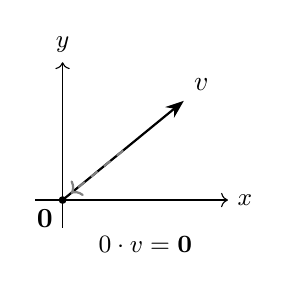
\begin{tikzpicture}[scale=0.7]
    \draw[axis] (-0.5,0) -- (3,0) node[right] {\small$x$};
    \draw[axis] (0,-0.5) -- (0,2.5) node[above] {\small$y$};
    \fill (0,0) circle (2pt) node[below left] {$\mathbf{0}$};
    \draw[vector, thick] (0,0) -- (2.2,1.8) node[above right] {$v$};
    \draw[->, thick, dashed, gray] (1.1,0.9) -- (0.15,0.12);
    \node at (1.5,-0.8) {\small $0 \cdot v = \mathbf{0}$};
\end{tikzpicture}

\small\textit{Scalar zero ``collapses'' any vector to the origin.}
\end{center}
\smallskip

\begin{tcolorbox}
\textbf{1.31 $a0 = 0$}

For every $a \in \F$, $a0 = 0$.
\end{tcolorbox}

\textbf{Proof:} For $a \in \F$:
\begin{align*}
    a0 &= a(0 + 0) \\
       &= a0 + a0
\end{align*}
Adding $-(a0)$ to both sides gives $0 = a0$. \hfill $\square$

\begin{tcolorbox}
\textbf{1.32 $(-1)v = -v$}

For every $v$ in a vector space, $(-1)v = -v$.
\end{tcolorbox}

\textbf{Proof:} For $v \in V$:
\begin{align*}
    v + (-1)v &= 1v + (-1)v \\
              &= (1 + (-1))v \\
              &= 0v \\
              &= 0
\end{align*}
This shows $(-1)v$ is an additive inverse of $v$. By uniqueness (1.27), $(-1)v = -v$. \hfill $\square$

\textbf{Key insight:} We can now write $-v$ as $(-1)v$. Subtraction is just a special case of scalar multiplication!

\smallskip
\begin{center}
\begin{tikzpicture}[scale=0.7]
    \draw[axis] (-2.5,0) -- (2.5,0) node[right] {\small$x$};
    \draw[axis] (0,-1.5) -- (0,1.5) node[above] {\small$y$};
    \fill (0,0) circle (1.5pt);
    \draw[vector] (0,0) -- (2,1) node[above right] {$v$};
    \draw[vector] (0,0) -- (-2,-1) node[below left] {$(-1)v = -v$};
    \draw[dotted] (-2.3,-1.15) -- (2.3,1.15);
\end{tikzpicture}

\small\textit{Scalar multiplication by $-1$ reverses direction.}
\end{center}
\smallskip

\begin{result}
\textbf{Summary of key results:}
\begin{itemize}
    \item $0v = 0$ (scalar zero times any vector is the zero vector)
    \item $a0 = 0$ (any scalar times the zero vector is the zero vector)
    \item $(-1)v = -v$ (the additive inverse is scalar multiplication by $-1$)
\end{itemize}
These three results connect the scalar and vector versions of ``zero'' and ``negative.''
\end{result}

%==============================================================================
\newpage
\section*{Non-Examples and Pitfalls}
%==============================================================================

Understanding what is \textit{not} a vector space is as important as knowing the definition. For each non-example, we identify the \textbf{specific axiom that fails}.

\smallskip
\begin{center}
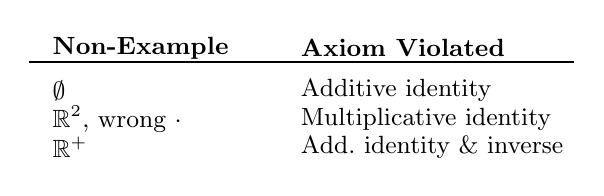
\begin{tikzpicture}[scale=0.9]
    % Table header
    \node[anchor=west, font=\bfseries\small] at (0,0) {Non-Example};
    \node[anchor=west, font=\bfseries\small] at (3.5,0) {Axiom Violated};
    \draw[thick] (-0.2,-0.2) -- (7.5,-0.2);
    % Row 1
    \node[anchor=west, font=\small] at (0,-0.6) {$\emptyset$};
    \node[anchor=west, font=\small] at (3.5,-0.6) {Additive identity};
    % Row 2
    \node[anchor=west, font=\small] at (0,-1.0) {$\R^2$, wrong $\cdot$};
    \node[anchor=west, font=\small] at (3.5,-1.0) {Multiplicative identity};
    % Row 3
    \node[anchor=west, font=\small] at (0,-1.4) {$\R^+$};
    \node[anchor=west, font=\small] at (3.5,-1.4) {Add.\ identity \& inverse};
\end{tikzpicture}

\small\textit{Quick reference: which axiom each non-example violates}
\end{center}
\smallskip

\begin{tcolorbox}[colframe=black!50]
\textbf{Non-Example: The Empty Set}

The empty set $\emptyset$ is not a vector space.

\textbf{Axiom violated:} \textit{Additive identity} --- there is no element $0 \in \emptyset$.

\textbf{Key point:} Every vector space must contain at least one element (the zero vector).
\end{tcolorbox}

\begin{tcolorbox}[colframe=black!50]
\textbf{Non-Example: $\R^2$ with ``wrong'' scalar multiplication}

Consider $\R^2$ with standard addition but scalar multiplication defined by:
\[
    \lambda(x, y) = (\lambda x, 0)
\]

\textbf{Axiom violated:} \textit{Multiplicative identity} ($1v = v$).

Check: $1(x, y) = (1 \cdot x, 0) = (x, 0) \neq (x, y)$ unless $y = 0$.

The operation ``forgets'' the second coordinate, so scaling by 1 doesn't preserve vectors.
\end{tcolorbox}

\begin{tcolorbox}[colframe=black!50]
\textbf{Non-Example: Positive Reals}

Consider $\R^+ = \{x \in \R : x > 0\}$ with standard addition and scalar multiplication.

\textbf{Axioms violated:}
\begin{itemize}
    \item \textit{Additive identity}: $0 \notin \R^+$ (zero is not positive)
    \item \textit{Additive inverse}: For $v = 1 \in \R^+$, we need $-1$, but $-1 \notin \R^+$
\end{itemize}

\textbf{Twist:} With different operations (multiplication as ``addition'' and exponentiation as ``scalar multiplication''), $\R^+$ \textit{can} be made into a vector space!
\end{tcolorbox}

%==============================================================================
\section*{Verifying Vector Space Axioms}
%==============================================================================

\begin{result}
\textbf{Strategy for proving $V$ is a vector space:}

\begin{enumerate}
    \item Define addition on $V$ (check it maps $V \times V \to V$).
    \item Define scalar multiplication (check it maps $\F \times V \to V$).
    \item Verify all 8 axioms.
\end{enumerate}

\textbf{Common shortcuts:}
\begin{itemize}
    \item If $V$ inherits operations from a known vector space (like $\F^n$ or $\F^S$), most axioms follow automatically.
    \item Commutativity and associativity often follow from the corresponding properties in $\F$.
\end{itemize}
\end{result}

\begin{result}
\textbf{Strategy for proving $V$ is NOT a vector space:}

Find ONE axiom that fails and provide a specific counterexample.

\textbf{Common failures:}
\begin{itemize}
    \item No additive identity ($0 \notin V$)
    \item No additive inverses ($-v \notin V$ for some $v$)
    \item Not closed under addition ($u + v \notin V$)
    \item Not closed under scalar multiplication ($\lambda v \notin V$)
    \item Multiplicative identity fails ($1v \neq v$)
\end{itemize}
\end{result}

\begin{tcolorbox}[colframe=black!50]
\textbf{Worked Example: Verifying $\F^2$ is a Vector Space}

Let's verify that $\F^2 = \{(x, y) : x, y \in \F\}$ with coordinate-wise operations is a vector space.

\textbf{1. Commutativity of addition:} Let $u = (u_1, u_2)$ and $v = (v_1, v_2)$.
\[
u + v = (u_1 + v_1, u_2 + v_2) = (v_1 + u_1, v_2 + u_2) = v + u \; \checkmark
\]
(using commutativity in $\F$)

\textbf{2. Additive identity:} The vector $0 = (0, 0)$ satisfies:
\[
(x, y) + (0, 0) = (x + 0, y + 0) = (x, y) \; \checkmark
\]

\textbf{3. Multiplicative identity:} For any $(x, y) \in \F^2$:
\[
1(x, y) = (1 \cdot x, 1 \cdot y) = (x, y) \; \checkmark
\]

\textbf{4. Distributive (scalar over sum):} Let $a \in \F$, $u, v \in \F^2$:
\[
a(u + v) = a(u_1 + v_1, u_2 + v_2) = (a(u_1 + v_1), a(u_2 + v_2))
\]
\[
= (au_1 + av_1, au_2 + av_2) = au + av \; \checkmark
\]

The remaining axioms (associativity of addition, associativity of scalar multiplication, additive inverses, other distributive law) follow similarly from properties of $\F$.
\end{tcolorbox}

%==============================================================================

\vfill
\begin{center}
\rule{0.5\linewidth}{0.4pt}

\textit{Key Takeaways}
\end{center}
\begin{enumerate}
    \item \textbf{Vector space axioms (CAAIMD$^2$):} 8 properties defining addition and scalar multiplication
    \item \textbf{Uniqueness:} Additive identity and inverses are unique
    \item \textbf{Key consequences:} $0v = 0$, $a0 = 0$, $(-1)v = -v$
    \item \textbf{Verification strategy:} Check all 8 axioms (or find one that fails for non-examples)
\end{enumerate}

\subsection*{Relevant Exercises}
Practice these problems from LADR to reinforce the material:
\begin{itemize}
    \item Section 1B: 1, 2, 3, 4, 5, 6
\end{itemize}

\begin{tcolorbox}[colframe=black!50]
\textbf{Common Problem Types:}
\begin{description}[style=nextline, leftmargin=1em, labelindent=0pt]
    \item[Prove a property from axioms]
    Start with one side. Apply axioms step-by-step. Justify each step by naming the axiom used.

    \item[Prove uniqueness]
    Assume two objects satisfy the definition. Show they must be equal using the defining property.

    \item[Verify a set is a vector space]
    Define operations clearly. Verify closure. Check all 8 axioms (use shortcuts when operations are inherited).

    \item[Show a set is NOT a vector space]
    Find one axiom that fails. Give a specific counterexample with explicit values.
\end{description}
\end{tcolorbox}

\end{document}
